% Results section. Meant to be \input into the final paper.
% Sources of truth: docs/FREEZE.md, experiments/LAYERS_V7_CLAIMS.md (H1--H6, test),
% experiments/LAYERS_RUNS.md (validation), docs/REFLECTED_FREEZE.md,
% experiments/REFLECTED_V1_RESULTS.md (R1--R4, test), experiments/REFLECTED_RUNS.md
% (validation findings 1--12). Every number below is copied from those files.
\providecommand{\todo}[1]{\textbf{[TODO:~#1]}}

\section{Results}
\label{sec:results}

\paragraph{Protocol.}
Probe results cover 19 checkpoints (18 base/retrieval models plus the XLM-R XL size control) under one plan. Places are split 60/20/20 into training, validation and test; layers and ridge penalties were selected on validation only. Before any test place was scored, we froze 169 cells (per model, dataset and pooling: the best validation layer of the \texttt{country-residual} probe on random-item, and the last layer) and six claims with pass criteria (H1--H6); the test split was then scored once. A claim requiring a 95\% block-bootstrap interval above 0 passes only if it holds for \emph{all three} seeds (and, where stated, on both splits). Claims about cosine similarity (R1--R4) were frozen afterwards and scored once on the same test cities: different claims about the same held-out data, fixed before that analysis read it. Anything outside a frozen claim is secondary. We mark held-out numbers \textbf{(test)} and exploration numbers \textbf{(validation)}; the latter are optimistic because layers and penalties were chosen on the same places. Gains are km over the training-only country centroid; positive means better than knowing the country.

\begin{table}[htb]
\centering
\footnotesize
\caption{Frozen probe claims on the held-out test split. A run is one model, split and seed. ``LB'' is the lower bound of the 95\% block-bootstrap interval. Criteria are as frozen in advance; H5 is descriptive.}
\label{tab:h-claims}
\begin{tabularx}{\linewidth}{@{}>{\raggedright\arraybackslash}p{0.27\linewidth}>{\raggedright\arraybackslash}X>{\raggedright\arraybackslash}p{0.25\linewidth}@{}}
\toprule
Claim & Criterion (test, every seed) & Outcome \\
\midrule
H1: decoders $\geq$4B hold within-country geography & \texttt{country-residual} LB $>0$, both splits; 8 models & \textbf{Supported}: 48/48 runs \\
H2: retrieval training keeps it & retrieval LB $>0$ in all 4 pairs; direction only if paired CIs exclude 0 on both splits & \textbf{Supported}; no direction in any pair \\
H3: MLM encoders up to 3.5B show none & each run LB $\leq 0$ or gain $<20$~km; 7 models & \textbf{Not supported}: 40/42 runs \\
H4: retrieval output vector beats the country & \texttt{sphere}, last layer, last token, random-item; 4 models & \textbf{Not supported}: 11/12 runs \\
H5: lat/lon $R^2$ mostly reflects the country & descriptive & all below centroid (0.95/0.98) \\
H6: not only famous places & smallest population quintile LB $>0$, both splits; 8 models & \textbf{Supported}: 16/16 \\
\bottomrule
\end{tabularx}
\end{table}

\subsection{Large decoders encode within-country geography}
\label{sec:res-decoders}

\paragraph{H1 (test).}
The \texttt{country-residual} probe is given the true country and predicts the offset from its training centroid, so it measures position \emph{within} a country. Every decoder from 4B up, base and retrieval-tuned, beats the country centroid on all 48 runs, by 116--375~km (Table~\ref{tab:h1-h3}). Test gains match validation (Qwen3-4B base, random-item: 120~km on validation, 118--146~km on test), so selecting layers on validation did not inflate them. The signal grows with Qwen3 size, and the Mistral-7B and Gemma-2-9B families, added to test whether the pattern is Qwen-specific, carry the most.
% Figure placeholder (validation, layers-v4; regenerate before use):
% \begin{figure}[t]\centering
% 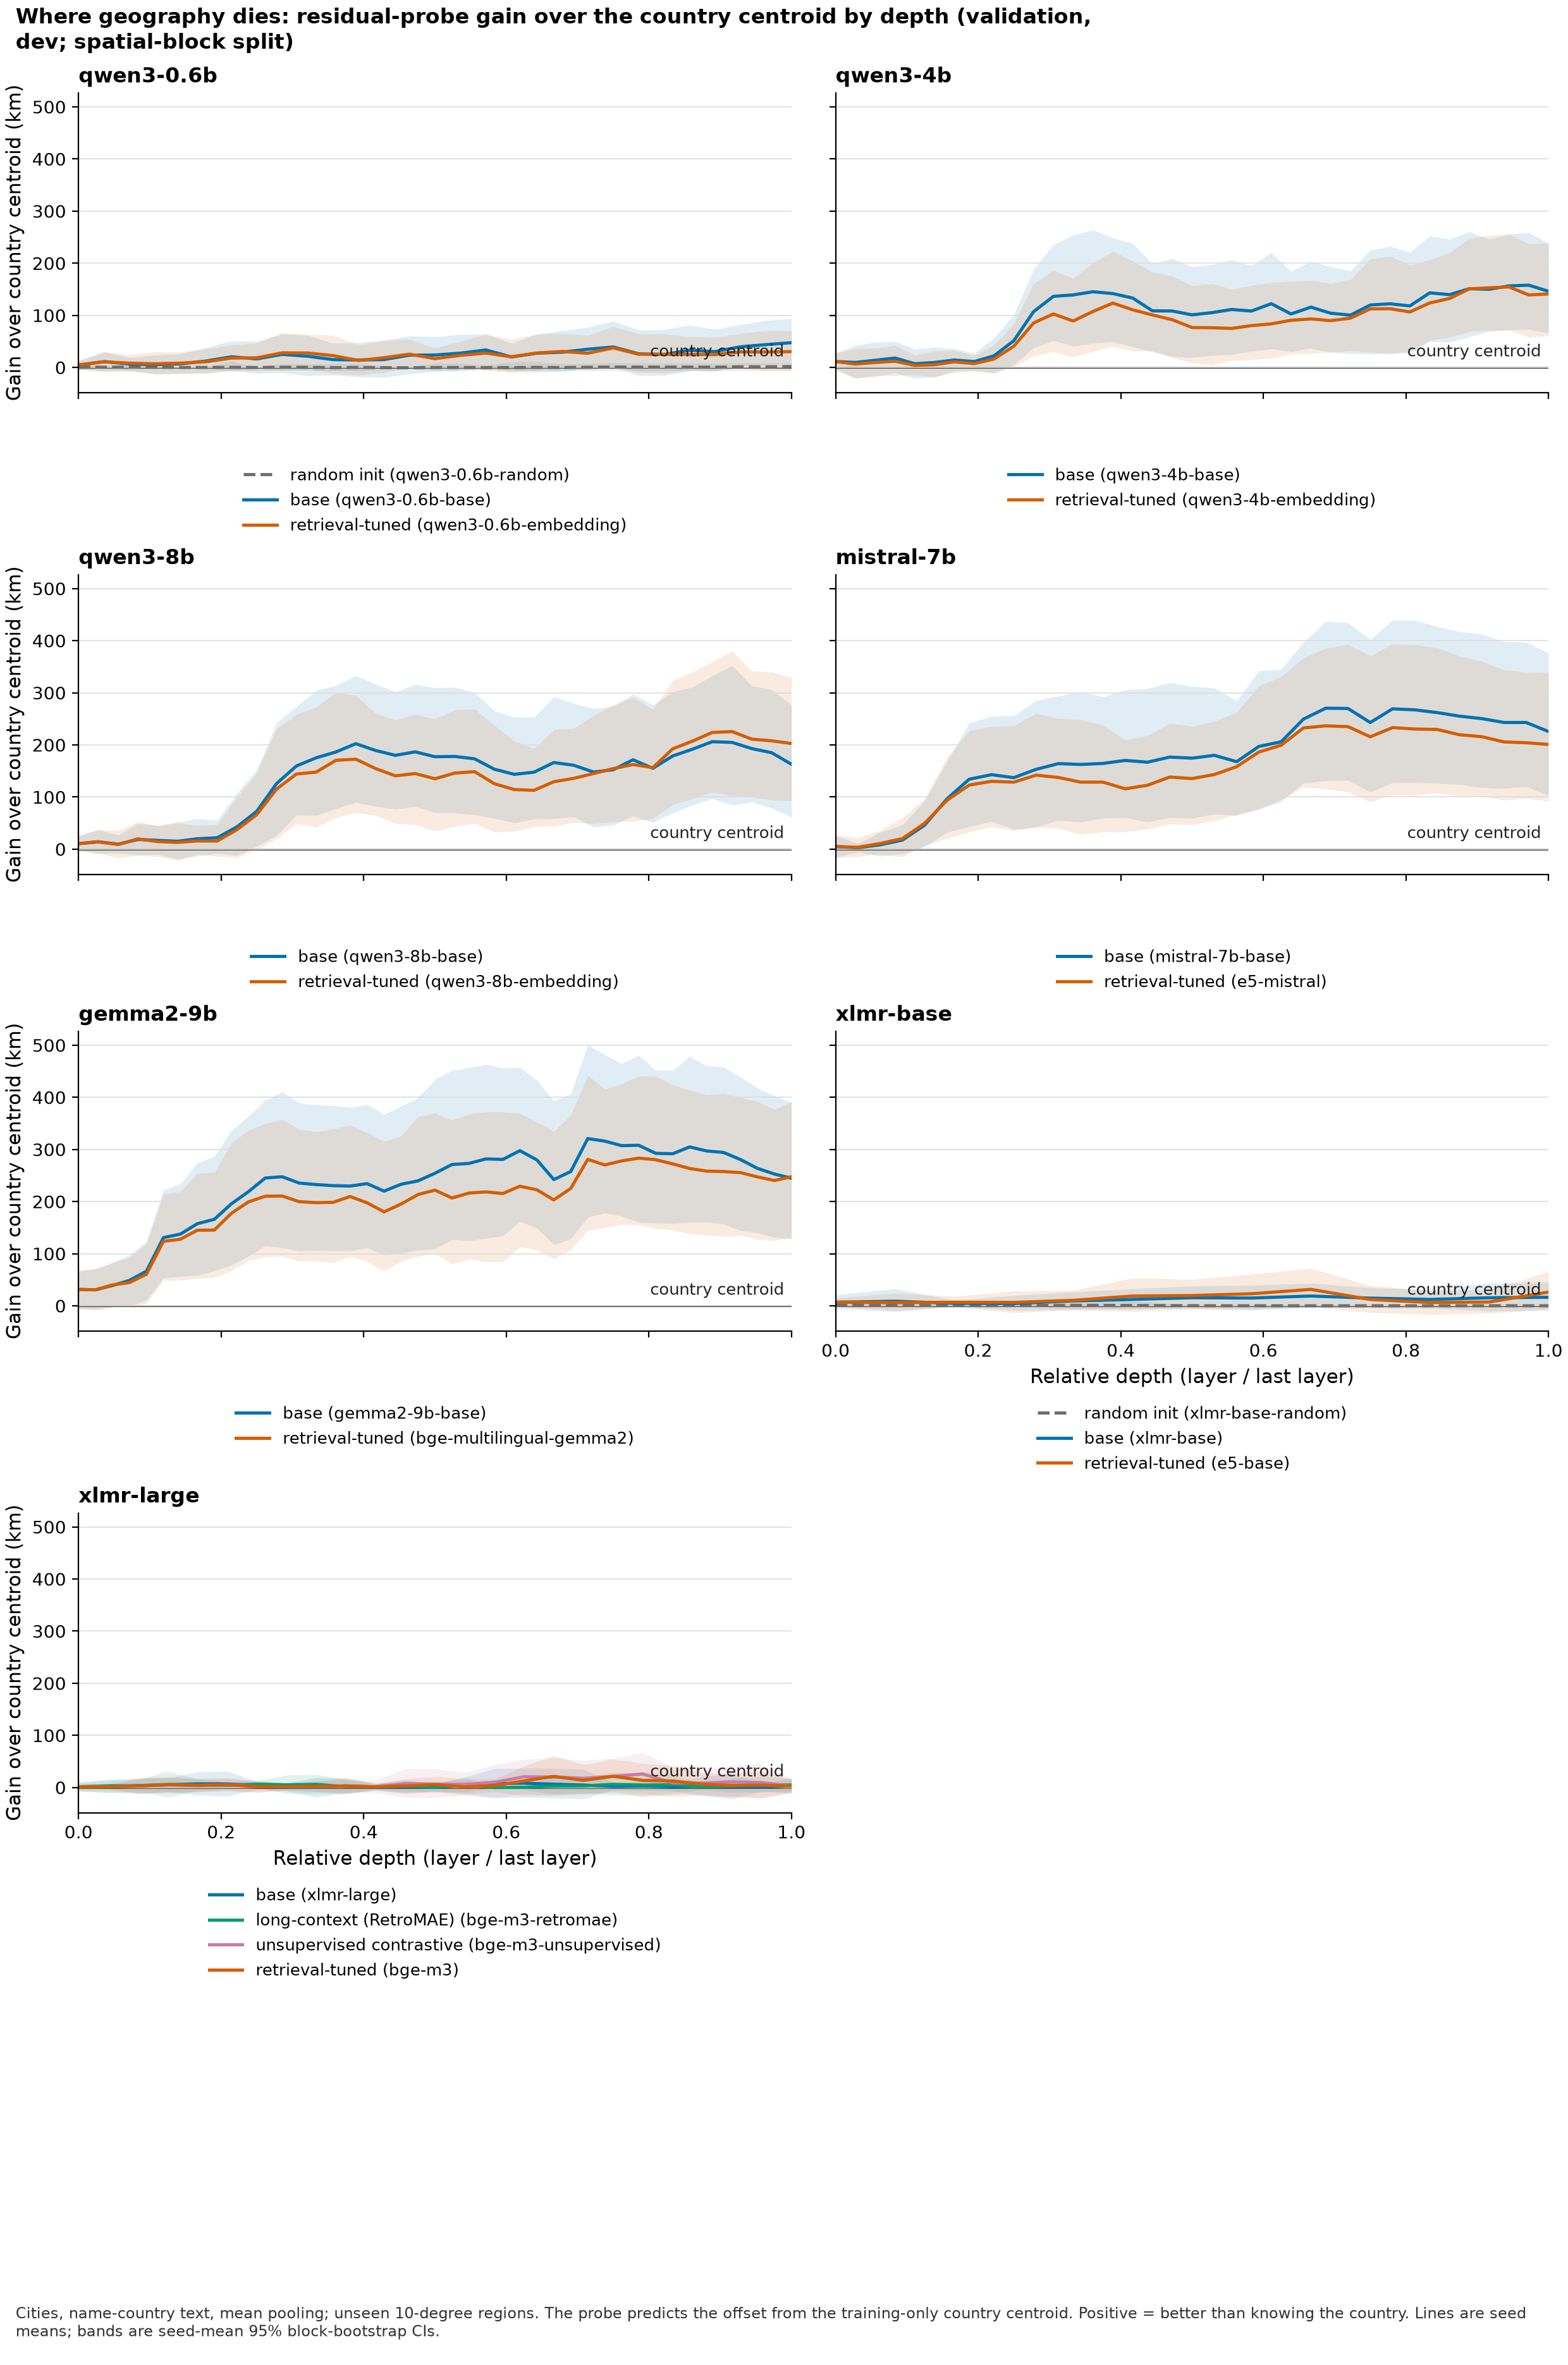
\includegraphics[width=\linewidth]{../docs/figures/layers-v4/where-geography-dies-residual.png}
% \caption{Country-residual gain by relative depth (validation).}\end{figure}

\begin{table}[t]
\centering
\footnotesize
\caption{\texttt{country-residual} gain over the country centroid (km) on the test split, cities \texttt{name-country}, mean pooling, frozen best-validation layer. Gains are the range over the three seeds; ``LB$>$0'' counts the six runs (2 splits $\times$ 3 seeds) whose interval lies above 0. Q1 is the smallest population fifth (seeds pooled, gain [95\% CI]); it was frozen for the H1 models only.}
\label{tab:h1-h3}
\begin{tabular}{@{}lrrrcrr@{}}
\toprule
Model & Layer & Spatial-block & Random-item & LB$>$0 & Q1 spatial-block & Q1 random-item \\
\midrule
\multicolumn{7}{@{}l}{\emph{Decoders (H1, H6)}} \\
Qwen3-4B-Base & 34 & 116--259 & 118--146 & 6/6 & 93 [47, 148] & 72 [19, 134] \\
Qwen3-Embedding-4B & 33 & 137--277 & 127--150 & 6/6 & 74 [32, 119] & 79 [33, 132] \\
Qwen3-8B-Base & 33 & 162--305 & 184--207 & 6/6 & 95 [33, 161] & 119 [57, 193] \\
Qwen3-Embedding-8B & 33 & 199--335 & 205--214 & 6/6 & 102 [54, 161] & 138 [82, 204] \\
Mistral-7B & 27 & 210--306 & 245--274 & 6/6 & 134 [69, 204] & 182 [104, 276] \\
e5-mistral & 25 & 243--306 & 239--263 & 6/6 & 131 [71, 197] & 168 [95, 256] \\
Gemma-2-9B & 35 & 259--375 & 296--325 & 6/6 & 193 [120, 270] & 224 [140, 320] \\
bge-multilingual-gemma2 & 33 & 277--367 & 272--304 & 6/6 & 189 [121, 261] & 211 [135, 301] \\
\midrule
\multicolumn{7}{@{}l}{\emph{Encoders (H3)}} \\
XLM-R base & 12 & 0--12 & $-5$--0 & 0/6 & & \\
multilingual-e5-base & 8 & 20--50 & 0--6 & 0/6 & & \\
XLM-R large & 3 & $-12$--6 & 0--1 & 0/6 & & \\
BGE-M3 (RetroMAE stage) & 16 & $-2$--20 & $-4$--3 & 0/6 & & \\
BGE-M3 (unsupervised stage) & 16 & 6--35 & 4--12 & 1/6 & & \\
BGE-M3 (final) & 16 & 6--41 & $-2$--4 & 0/6 & & \\
XLM-R XL (3.5B) & 32 & 0--31 & $-1$--12 & 1/6 & & \\
\bottomrule
\end{tabular}
\end{table}

\paragraph{H6 (test): small towns too.}
For every H1 model, the smallest population fifth of cities still has a gain interval above 0 on both splits: 72--224~km, lower bounds 19--140~km (Table~\ref{tab:h1-h3}). Popularity modulates the signal (validation): the largest fifth gains about 1.5--3 times more (Qwen3-4B base, random-item: 60 vs.\ 181~km), and the 0.6B Qwen3 models gain only on the largest cities. Quintiles also differ in geography, so this gradient is descriptive.

\paragraph{H5 (test): latitude/longitude $R^2$ mostly measures the country.}
\citet{gurnee2024space} report $R^2$ of probes onto latitude and longitude. On \texttt{name-country} text the country centroid alone gives $R^2=0.95$/0.98 (lat/lon). Every model at its frozen layer is below this (trained models 0.79--0.93/0.88--0.95), and probes on \emph{randomly initialised} networks reach 0.79/0.87 (Qwen3-0.6B) and 0.74/0.83 (XLM-R base). High lat/lon $R^2$ is thus reachable from tokenisation and the country name, and is not evidence of within-country knowledge; hence our headline measure is the country-residual gain, on which the random-init controls, in the spirit of control tasks \citep{hewitt2019control}, gain only 1--4~km (validation).
% Test random-init country-residual gains at their frozen layers are not in LAYERS_V7_CLAIMS.md.
% At the last layer (REFLECTED_V1_RESULTS.md, probe column) they lie between -8 and 0 km.
Raw-output $R^2$ is also fragile (validation): at layer~6 of Qwen3-Embedding-4B, ``Carcassonne, France'' has a hidden-state norm of 776 (median 32), the ridge maps it to about $(-1866, 2863)$ degrees, and latitude $R^2$ is $-0.14$ with this city evaluated and 0.84 without it. We therefore froze $R^2$ on predictions clipped to valid coordinates as primary; at the frozen test layers clipping changes nothing. Kilometre metrics are barely affected.
% Figure placeholder (validation): ../docs/figures/layers-v4/r2-by-depth.png

\subsection{Encoders: small gains, not explained by size}
\label{sec:res-encoders}

\paragraph{H3 (test) failed narrowly.}
H3 required every encoder run to have an interval reaching 0 or a gain under 20~km. Forty of 42 runs do; two spatial-block runs do not, so the claim is not supported: the unsupervised BGE-M3 stage (35 [5, 66]~km) and XLM-R XL (20 [4, 39]~km), both seed 1729. (The validation dry run had already failed H3 on spatial-block, for XLM-R base and multilingual-e5-base.) On random-item every encoder is within 12~km of 0; spatial-block holds out whole 10$^\circ$ blocks, where the training centroid is biased and weak probes can beat it. The data support a gap in magnitude, not ``none'': no encoder run exceeds 50~km, no 4B+ decoder run is below 116~km (Table~\ref{tab:h1-h3}), and nearest neighbours find a small encoder signal (Section~\ref{sec:res-crossover}).

\paragraph{Size control (validation, with test check).}
The paired encoders have at most 0.56B parameters and the decoders with a clear signal at least 4B, so the contrast is confounded with size. XLM-R XL (3.5B) behaves like the small encoders, not like a 4B decoder (Table~\ref{tab:xl}; validation random-item 5.8 vs.\ 119.6~km), while among decoders size does matter (Qwen3-0.6B: 11.8~km). Size alone does not explain the encoder result, but architecture is not isolated: encoders and decoders also differ in pretraining objective and data.

\begin{table}[t]
\centering
\footnotesize
\caption{Encoder size control: \texttt{country-residual} gain (km), cities \texttt{name-country}, mean pooling. Validation: seed mean at the best validation layer for that split; brackets span the three seeds' 95\% intervals. Test: range over seeds at the frozen layer (chosen on validation random-item and used for both splits). n/r: not among the frozen claim tables.}
\label{tab:xl}
\begin{tabular}{@{}lrllrr@{}}
\toprule
& & \multicolumn{2}{c}{Validation} & \multicolumn{2}{c}{Test (frozen layer)} \\
\cmidrule(lr){3-4}\cmidrule(l){5-6}
Model & Params & Random-item & Spatial-block & Random-item & Spatial-block \\
\midrule
XLM-R large & 0.56B & 1.2 [$-4.2$, 11.1] (L3) & 8.2 [$-23.1$, 57.0] (L15) & 0--1 & $-12$--6 \\
BGE-M3 & 0.56B & 10.6 [$-10.2$, 36.3] (L16) & 21.4 [$-11.1$, 81.4] (L18) & $-2$--4 & 6--41 \\
XLM-R XL & 3.5B & 5.8 [$-8.1$, 21.6] (L32) & 18.4 [$-13.4$, 51.3] (L21) & $-1$--12 & 0--31 \\
Qwen3-0.6B-Base & 0.6B & 11.8 [$-9.7$, 38.5] (L24) & 47.5 [0.2, 159.4] (L28) & n/r & n/r \\
Qwen3-4B-Base & 4B & 119.6 [61.8, 204.5] (L34) & 157.9 [62.7, 315.5] (L35) & 118--146 & 116--259 \\
\bottomrule
\end{tabular}
\end{table}

\subsection{Retrieval training keeps geography decodable}
\label{sec:res-retrieval}

\paragraph{H2 (test).}
In all four 4B+ pairs (Qwen3-4B, Qwen3-8B, Mistral-7B$\to$e5-mistral, Gemma-2-9B$\to$bge-multilingual-gemma2) the retrieval model's gain interval is above 0 on every run, so retrieval training keeps within-country geography decodable. A directional claim required all three seeds' paired retrieval-minus-base intervals (over shared 10$^\circ$ blocks) to exclude 0 on the same side on both splits; no pair qualifies. The only consistent difference is Gemma on random-item, where bge-multilingual-gemma2 is 21--31~km below its base on all seeds (e.g.\ $-25$ [$-43$, $-6$]); spatial-block does not confirm it ($-37$ [$-81$, 2], $-9$, $+18$). Every other paired interval includes 0 (estimates $-37$ to $+37$~km). The secondary pairs (Qwen3-0.6B and the two encoder pairs) show no passing retrieval gain and no direction.
% Station and name-only results were scored on test as secondary cells but are not summarised
% in the sources. Validation only: Qwen3-8B stations random-item 170 (base) vs 179 (retrieval).
\todo{add secondary test results for stations and \texttt{name}-only text if reported.}

\paragraph{H4 (test): the search vector itself.}
H4 asked whether a plain \texttt{sphere} probe on the vector a retrieval model searches with (last layer, last token) beats the country centroid. Qwen3-Embedding-8B, e5-mistral and bge-multilingual-gemma2 do on every seed (332--451~km); Qwen3-Embedding-4B does on two (252 [46, 527], 286 [49, 560]) but not the third (193 [$-55$, 476]), so H4 fails under the all-seeds rule. The mean-pooled encoder retrieval models (secondary) are far below the centroid ($-610$ to $-787$~km). BGE-M3 searches with its CLS token, which we did not extract.

\subsection{Is the geography reflected in cosine similarity?}
\label{sec:res-reflected}

Probes show that information is \emph{decodable}; retrieval uses cosine similarity. We ask whether a city's cosine nearest neighbours are close \emph{within its country}. Per country with at least 30 evaluated cities, kNN gain is $1-\bar d_{10}/\bar d_{\mathrm{all}}$: mean distance to the 10 most cosine-similar same-country cities over mean distance to all same-country cities, averaged and bootstrapped over countries. Zero is random; true distances give a ceiling of 0.733--0.746 (test). Character $n$-gram TF-IDF and a shuffled-position null score 0 (validation), so the effect is not surface form. We use last-layer vectors of \texttt{name-country} cities; centring uses training cities only.

\begin{table}[t]
\centering
\footnotesize
\caption{Reflected geography on the test cities (random-item split, last layer). kNN gain under raw cosine (range over three seeds; ceiling 0.733--0.746) and the retrieval-minus-base difference paired by country. R1 required all 48 intervals (4 pairs $\times$ 2 poolings $\times$ \{raw, centred\} $\times$ 3 seeds) to lie above 0.}
\label{tab:r1}
\begin{tabular}{@{}llccccc@{}}
\toprule
& & \multicolumn{2}{c}{kNN gain (raw cosine)} & \multicolumn{2}{c}{Paired difference} & Intervals \\
\cmidrule(lr){3-4}\cmidrule(lr){5-6}
Pair & Pooling & Base & Retrieval & Raw & Centred & above 0 \\
\midrule
Qwen3-4B & mean & 0.057--0.063 & 0.103--0.110 & +0.040--0.054 & +0.055--0.056 & 6/6 \\
         & last & 0.018--0.024 & 0.104--0.119 & +0.080--0.101 & +0.086--0.109 & 6/6 \\
Qwen3-8B & mean & 0.063--0.073 & 0.132--0.144 & +0.060--0.074 & +0.071--0.075 & 6/6 \\
         & last & 0.021--0.027 & 0.125--0.144 & +0.098--0.118 & +0.104--0.114 & 6/6 \\
Mistral-7B$\to$e5-mistral & mean & 0.125--0.132 & 0.142--0.157 & +0.017--0.028 & +0.008--0.018 & 5/6 \\
         & last & 0.043--0.051 & 0.245--0.274 & +0.194--0.224 & +0.201--0.228 & 6/6 \\
Gemma-2-9B$\to$bge-mult.-gemma2 & mean & 0.172--0.184 & 0.185--0.213 & +0.013--0.029 & +0.026--0.042 & 5/6 \\
         & last & 0.168--0.179 & 0.196--0.211 & +0.028--0.032 & +0.033--0.037 & 6/6 \\
\midrule
\multicolumn{6}{@{}l}{Total} & 46/48 \\
\bottomrule
\end{tabular}
\end{table}

\paragraph{R1 (test) failed its strict rule.}
R1 claimed that retrieval models' output vectors reflect within-country geography in cosine more than their bases' output vectors, with all 48 paired intervals above 0. Forty-six are (Table~\ref{tab:r1}). Both misses are mean-pooled, seed 3141: Mistral$\to$e5-mistral with centred cosine ($+0.008$ [$-0.006$, $+0.022$]) and Gemma$\to$bge-multilingual-gemma2 with raw cosine ($+0.013$ [$-0.006$, $+0.032$]). Every point estimate is positive, and all 24 last-token and all Qwen3 comparisons pass. The supported statement: at last-token pooling, which these retrieval models use for search, the retrieval output vector reflects within-country geography more than the base's in all four pairs; at mean pooling the difference is smaller and, for Mistral and Gemma, not significant on every seed. The largest change is Mistral to e5-mistral at the last token (0.043--0.051 to 0.245--0.274). The 0.6B and encoder pairs (secondary) differ by at most 0.031.

\paragraph{Not an isotropy artefact (validation, test).}
Anisotropy could hide geography from raw cosine in base models. On validation, centring or removing the top five principal components \citep{mu2018allbutthetop} (fit on training cities) raises base-model kNN gain only modestly (Qwen3-8B base, mean: 0.07 to 0.10). After all-but-the-top the retrieval advantage remains at the last token for Qwen3-4B, Qwen3-8B and Mistral, but for Gemma it shrinks to about $+0.01$ with intervals spanning 0. Centred cosine was part of the frozen R1 test, where every last-token comparison passes.

\paragraph{R2 (test): it is partial.}
The best model, e5-mistral (last token), reaches 0.245--0.274 of a 0.733--0.746 ceiling, about one third; bge-multilingual-gemma2 reaches 0.196--0.211, Qwen3-Embedding-8B 0.125--0.144 and Qwen3-Embedding-4B 0.104--0.119 (last token). Encoders and random-init controls are at 0.01--0.05 (XLM-R XL 0.025--0.048).

\paragraph{Where the difference arises (validation only).}
R1 compares output vectors only. Computing centred-cosine kNN gain at every layer (Table~\ref{tab:depth}; validation, not frozen) separates two mechanisms. With mean pooling, base models' best intermediate layers already reflect within-country geography about as well as the retrieval models (Gemma-2-9B 0.240 vs.\ 0.234), and lose much of it in the final layers (Qwen3-8B 0.131 to 0.084; Gemma 0.240 to 0.177), whereas retrieval models keep it to the output: retrieval training mostly \emph{preserves} what the base discards. With last-token pooling, the base model's last token barely reflects geography at any depth (except Gemma's final layers), while the retrieval model's does from mid-depth on (Mistral: at most 0.061 vs.\ 0.308): here retrieval training \emph{creates} it, consistent with embedding training making the last token a summary of the text. \citet{jiang2026layerwise} compare embedders and base LLMs layer by layer; this profile adds a geographic, similarity-based view. The test-level claim remains about output vectors.

\begin{table}[t]
\centering
\footnotesize
\caption{Depth profile of centred-cosine kNN gain (validation, mean of three seeds). ``Best'' is the maximum over layers (layer in parentheses); ``last'' is the output layer.}
\label{tab:depth}
\begin{tabular}{@{}llcccc@{}}
\toprule
& & \multicolumn{2}{c}{Base} & \multicolumn{2}{c}{Retrieval} \\
\cmidrule(lr){3-4}\cmidrule(l){5-6}
Pair & Pooling & Best (layer) & Last & Best (layer) & Last \\
\midrule
Qwen3-4B & mean & 0.094 (32) & 0.064 & 0.106 (36) & 0.106 \\
         & last & 0.038 (20) & 0.024 & 0.118 (32) & 0.113 \\
Qwen3-8B & mean & 0.131 (32) & 0.084 & 0.145 (36) & 0.145 \\
         & last & 0.050 (23) & 0.030 & 0.161 (32) & 0.141 \\
Mistral-7B$\to$e5-mistral & mean & 0.194 (27) & 0.130 & 0.219 (26) & 0.147 \\
         & last & 0.061 (12) & 0.044 & 0.308 (26) & 0.259 \\
Gemma-2-9B$\to$bge-mult.-gemma2 & mean & 0.240 (38) & 0.177 & 0.234 (35) & 0.216 \\
         & last & 0.181 (41) & 0.177 & 0.245 (32) & 0.217 \\
XLM-R large$\to$BGE-M3 & mean & 0.048 (7) & 0.034 & 0.046 (14) & 0.041 \\
\bottomrule
\end{tabular}
\end{table}

\subsection{Probes versus nearest neighbours}
\label{sec:res-crossover}

We also predict each test city's position as the mean of its 10 most cosine-similar same-country training cities (last layer) and score it like the probe.

\paragraph{R3 (test, descriptive): a crossover inside known regions.}
On random-item, nearest neighbours beat the probe for every retrieval model at the last token (12 of 12 runs; 7 with the paired interval above 0; e.g.\ e5-mistral by 39--48~km), and the probe beats nearest neighbours for every base model at mean pooling (12 of 12; 8 significant; by 13--62~km). The interaction, retrieval minus base of (probe error $-$ neighbour error) paired by place, is positive in all 24 runs (4 pairs $\times$ 2 poolings $\times$ 3 seeds) and significant in 19 (validation: 17); it is largest for Mistral at the last token (+138 to +156~km). For retrieval models, probe gains thus understate the geography present. Neighbours also find a small encoder signal the probe misses: XLM-R XL reaches 33--40~km (all intervals above 0) where its probe is within 8~km of 0; random-init controls stay within 7~km of 0.

\paragraph{R4 (test, descriptive): neighbours cannot extrapolate.}
On spatial-block, the probe beats nearest neighbours for every base model (12 of 12 at mean pooling, all significant; by 97--179~km) and in 10 of 12 retrieval-model runs at the last token (the two exceptions span 0). The interaction is positive in 19 of 24 runs but significant in only 6, and significantly negative in one (Gemma, last token, seed 1729). Neighbours can only point to places seen in training, whereas a linear map can extrapolate: the retrieval-model advantage holds for unseen cities in known regions, not for unseen regions.

\subsection{Negative result: a probe-based fix}
\label{sec:res-fix}

We tested a cheap fix (validation cities, seed 1729 only; exploratory, not frozen). A ridge probe from the normalised last-layer vector to the unit-sphere position, fit on training cities, was applied unchanged to all 11,833 stations by amplifying its three-dimensional subspace by $1+b$. With $b=10$, the mean distance to a station's 10 cosine neighbours falls for all four 4B+ retrieval models (e.g.\ Qwen3-Embedding-8B: 1,446 to 1,033~km). But appending the station's country centroid, read from its country code ($w=0.1$), lowers it further in every model (652--845 vs.\ 770--1,033~km) at about the same genre-agreement cost (Qwen3-Embedding-4B: 0.538 vs.\ 0.537, from 0.554). The probe fix mainly corrects a neighbour's country; within countries it barely changes city neighbourhoods (kNN gain $+0.003$ to $+0.014$), because the probe's positions are less locally accurate than cosine already is. Appending true coordinates ($w=0.2$, a perfect geocoder) is far stronger (434--617~km). The fix is dominated by a trivial country baseline, and we do not claim it. The few-seed projection of \citet{feuerstein2026recovering} is the natural baseline for any learned fix; we have not run it.
\todo{decide whether to run the projection of \citet{feuerstein2026recovering} as a baseline.}

\subsection{Closing the gap}
\label{sec:res-closing}
% Sources: experiments/FIX_RUNS.md (selection, validation), docs/FIX_FREEZE.md (claims), experiments/FIX_V1_RESULTS.md (test, run once, job 3325420).

We tried coordinate-free changes to frozen retrieval models that do not require a geocoder at query or index time. All components are fit on training cities. We selected them on validation cities, using stations as a transfer and cost check (no station is used for fitting). Station genre agreement measures semantic cost: the share of a station's ten neighbours that share a genre tag. The country-code baseline cannot change within-country structure by construction.

Three components help, and they combine.
(i) \emph{Layer fusion}: adding the centred cosine of an intermediate layer, chosen on training cities (e5-mistral layers 25--26, bge-multilingual-gemma2 layer 32), improves within-country neighbours and genre agreement together.
(ii) \emph{A distance probe}: a rank-32 linear map trained on training cities with a triplet loss (anchor, one of its ten nearest same-country cities, a random same-country city), in the spirit of structural probes; its squared distance is subtracted from the cosine score. Unlike the 3-D position probe, it targets neighbour ranking within countries. It also improves stations whose texts it was never fit on, and it holds when whole 10$^\circ$ regions are held out.
(iii) \emph{A task instruction} on both sides (native format; ``Given the name of a place, retrieve places that are geographically closest to it''). A generic instruction (``\ldots retrieve semantically similar text'') has the opposite effect: it lowers within-country geography below the uninstructed vector and raises genre agreement. The instruction therefore steers which facet cosine similarity tracks. All three geographic wordings we tried move in the same direction, with magnitudes that depend on wording.

\begin{table}[t]
\centering
\footnotesize
\setlength{\tabcolsep}{3.5pt}
\caption{Coordinate-free fixes on held-out test cities (run once; settings chosen on validation). City columns are within-country kNN gain (ceiling about 0.74) for random-item (RI) and spatial-block (SB) splits. Genre is station genre agreement; STS is Spearman correlation on STS-Benchmark test, a set not used for selection. Means over three seeds. Genre and STS are shown for RI.}
\label{tab:fixes}
\begin{tabular}{@{}lcccccccc@{}}
\toprule
& \multicolumn{4}{c}{e5-mistral} & \multicolumn{4}{c}{bge-multilingual-gemma2} \\
\cmidrule(lr){2-5}\cmidrule(lr){6-9}
Method & RI & SB & Genre & STS & RI & SB & Genre & STS \\
\midrule
Cosine (output) & 0.256 & 0.260 & 0.520 & 0.845 & 0.202 & 0.232 & 0.511 & 0.822 \\
Country-code append ($w=0.1$) & 0.256 & 0.260 & 0.511 & -- & 0.202 & 0.232 & 0.497 & -- \\
Layer fusion + distance probe & 0.321 & 0.326 & 0.536 & 0.863 & 0.276 & 0.302 & 0.540 & 0.844 \\
Geography instruction & 0.333 & 0.345 & 0.515 & 0.859 & 0.275 & 0.291 & 0.521 & 0.860 \\
Instruction + fusion + probe & \textbf{0.370} & \textbf{0.382} & 0.516 & 0.858 & \textbf{0.345} & \textbf{0.364} & 0.523 & 0.846 \\
\midrule
Geocoder oracle ($w=0.2$) & 0.307 & 0.295 & 0.505 & -- & 0.246 & 0.261 & 0.492 & -- \\
\bottomrule
\end{tabular}
\end{table}

Before running the test we froze two claims for e5-mistral and bge-multilingual-gemma2 (two splits, three seeds each). First, the full fix improves city within-country kNN gain over cosine, paired by country, with a 95\% bootstrap interval above zero. Second, STS-Benchmark test Spearman drops by at most 0.03. Both held in all twelve runs (Table~\ref{tab:fixes}).

Within-country neighbour quality rose from 0.20--0.26 to 0.35--0.38, from about one third of the ceiling to about one half. Paired differences were $+0.105$ to $+0.149$, and the lowest interval bound was $+0.084$.

STS did not fall; it rose by 0.013--0.028. This rise is probably an effect of using any instruction rather than geography: the cosine baseline is uninstructed, and both models are usually used with one. For bge-multilingual-gemma2, fusion and probe cost some STS relative to the instruction alone (0.846 vs 0.860). Genre agreement moved by at most 0.016.

On cities, the fix exceeds a blend with true coordinates ($w=0.2$). On stations, the geocoder remains ahead (0.257 vs 0.231 for e5-mistral; 0.253 vs 0.247 for bge-multilingual-gemma2).

The fix does not transfer for free. Qwen3-Embedding-8B also gains on cities in all six runs ($+0.077$ to $+0.121$), but its station genre agreement falls by about 0.10 and its STS by about 0.02.
\todo{Compare with the projection of \citet{feuerstein2026recovering}; contrast with training-time location embeddings \citep{srinivasagan2026location}; an STS-instruction baseline would separate the any-instruction effect from geography.}
